\chapter{Praktische Evaluation}

\section{Experimentelle Umgebung}
Die folgenden Experimente wurden auf Ubuntu 24.04 auf einem Rechner mit 16 ???? Prozessoren und 128GB RAM durchgeführt. Die C++-Implementierung wurde
mithilfe von GCC in der Version 13.1 kompiliert.

\section{Implementierung}
Die Implementierung der Algorithmen erfolgte im C++20-Standard.

\section{Daten}
Die Experimente wurden auf verschiedenen Datenbausteinen vom Pizza \& Chili-Corpus durchgeführt. Die verwendeten Datenbausteine sind in der folgenden Tabelle aufgelistet.

\begin{center}
    \begin{tabular}{|c|c|c|c|c|}
        \hline
        \textbf{Datei} & \textbf{Größe} & \textbf{Alphabet} & \textbf{Beschreibung} \\
        \hline
        \hline
        \texttt{dna} & 100MB & 4 & DNA-Sequenzen \\
        \hline
        \texttt{english} & 100MB & 256 & Englische Texte \\
        \hline
        \texttt{proteins} & 100MB & 20 & Proteinsequenzen \\
        \hline
        \texttt{sources} & 100MB & 256 & Quellcode \\
        \hline
        \texttt{xml} & 100MB & 256 & XML-Dateien \\
        \hline
    \end{tabular}
\end{center}
Es handelt sich hierbei um Präfixe der Originaldateien, die im Pizza \& Chili-Corpus enthalten sind.

\section{Ergebnisse}
Die Ergebnisse der Experimente sind in den folgenden Tabellen und Abbildungen dargestellt.\\
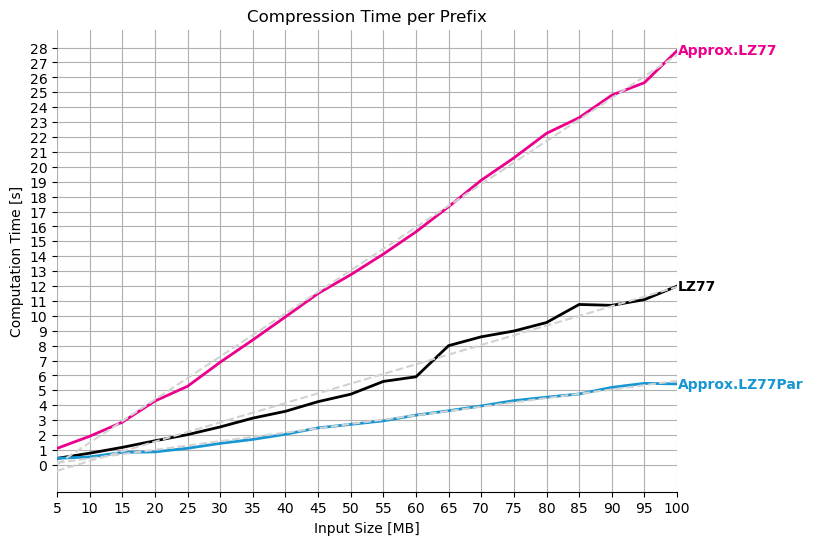
\includegraphics[scale = 0.65]{bilder/progressive.png}\\
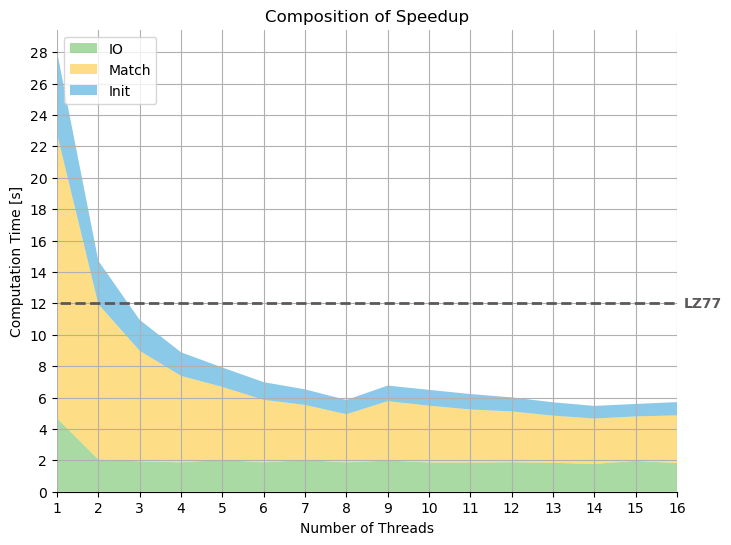
\includegraphics[scale = 0.65]{bilder/progressive_speedup_stack.png}\\
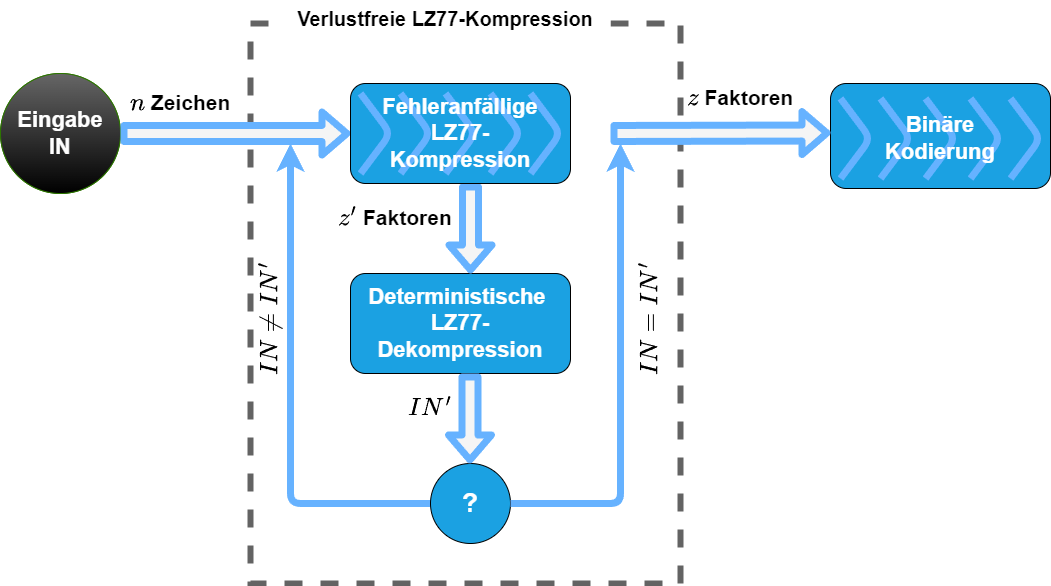
\includegraphics[scale = 0.4]{bilder/lasvegas_algorithm.png}